\documentclass[a4paper, 12pt]{report}

\title{Editeur Web}
%% Pour la police de caractères.
\usepackage{fontspec}
%% Pour la langue des titres et sous-titres.
\usepackage[francais]{babel}
%% Pour de belles images.
\usepackage{graphicx}
%% Pour des marges plus équitables.
\usepackage[margin=2cm]{geometry}
%% Pour faire le glossaire.
\usepackage[xindy]{glossaries}
\makeglossaries
%% La police de caractères.
\setmainfont{Delicious-Roman}
%% Pour pouvoir écrire du code.
%\usepackage{minted}
%\usemintedstyle{tango}
\begin{document}
	\begin{titlepage}
		\center{
\includegraphics[width=5cm]{images/logoUM2.png}}	\\ 
		~\\
		~\\
		~\\
		~\\
		~\\		
		\begin{center}
			{\large Rapport préliminaire de projet} \\
			{\large Licence 3}\\
			\vspace{1,5cm}
			{\Huge Editeur de sites web}\\
			~\\
			~\\
			~\\
			
\includegraphics[width=12.5cm]{images/logoTest1.png}
			~\\
			~\\
			{\large Réalisé par :} \\
			~\\
			{\LARGE Pierre Burc, Olivier Duplouy, \\
				      Hamza Erraji, Issame Amal,\\
				      Mickaël Berger, Joachim Divet,\\
				      Zaydane Sadiki et Abdelhamid Belarbi}\\
			\vspace{1,5cm}
			{\large Sous la direction de :} \\
			~\\
			{\LARGE Michel Meynard} \\
			\vspace{2.5cm}
			{\large Année universitaire 2011-2012}			
		\end{center}
	\end{titlepage}
%%%%%%%%%%%%%%%%%%%%%%%%%%%%%%%%%%%%%%%%%%%%%%%%%%%%%%%%%%%%%%%%%%%%%%%%%%%%%%%%%%%%%%%%%%%%%%%%%%%%%%%%%%%%%%%%%%%%%%%%%%%%%%%%%%
%%%%%%%%%%%%%%%%%%%%%%%%%%%%%%%%%%%%%%%%%%%%%%%%%%%%%%%%%%%%%%%%%%%%%%%%%%%%%%%%%%%%%%%%%%%%%%%%%%%%%%%%%%%%%%%%%%%%%%%%%%%%%%%%%%
\begin{chapter}*{Avant-propos}
	Il serait profondément malsain de commencer la description de ce projet sans une touche de présentation avant cela.\\
	Nous sommes donc huit étudiants de la Faculté des sciences de Montpellier, dans le domaine de l'informatique.
	Nous fûmes réunis pour la première fois en janvier 2012 pour débattre sur le sujet de notre projet, à savoir :\\ 
	\quotation{\emph{"Dans le cadre du développement de sites web, on souhaiterait utiliser un éditeur multi-fichiers permettant de réaliser différentes actions sur des fichiers relatifs à un site."}}\\


    Après cette réunion nous avons à force de discussions, d'argumentations opposées, d'idées nouvelles et de feuilles de papier, décidés d'une 
    marche à suivre pour répondre à cette problématique.\\
    Et c'est ainsi que dans les pages qui vont suivre sont exposées nos conclusions quant à la mise en place d'une solution.	
\end{chapter}

	\begin{part}{Conception}
		\begin{chapter}{Analyse de l'existant}
			\begin{section}{Espresso}
				\begin{figure}[h]
					\begin{center}
						
\includegraphics[width=3cm]{images/logoEspresso.png}
						\caption{Espresso}
					\end{center}
				\end{figure}~\\
				Le premier programme d'édition de site web que nous avons étudié, il propose les mêmes fonctionnalités que le
				logiciel que nous nous proposons de développer, à savoir coloration syntaxique, indentation automatique, arborescence des codes, etc.
				Il sera à priori une bonne source d'inspiration pour nous d'autant plus que l'interface est très soignée et agréable d'utilisation.
			\end{section}
			~\\
			\begin{section}{Aptana}
				\begin{figure}[h]
					\begin{center}
						
\includegraphics[width=4cm]{images/logoAptana.png}
						\caption{Aptana}
					\end{center}
				\end{figure}~\\
				Cet éditeur propose un ensemble de fonctionnalités nombreuses et variées. Beaucoup plus fourni que Espresso, il propose des fonctionnalités complexes dans divers langages : déboguage, déploiement automatique, gestionnaire de version inclus, terminal intégré et moult autres outils.
				Pour nous c'est un bon modèle à suivre en évitant tout de même de tomber dans le piège du sur-nombre d'options qui importuneraientt l'utilisateur. 
			\end{section}
			~\\
			\begin{section}{Dreamweaver}
				\begin{figure}[h]
					\begin{center}
						
\includegraphics[width=3cm]{images/logoDreamweaver.png}
						\caption{Dreamweaver}
					\end{center}
				\end{figure}~\\
				Dreamweaver est une référence en la matière. Il réunit les atouts des deux éditeurs sus-cités en joignant l'utile à l'agréable.
				Il possède en outre un mode dit WYSIWYG. Derrière ce sigle barbare se cache la possibilité intéressante de dessiner l'interface d'un site web.
				Nous concernant, nous pourrons proposer à l'utilisateur de visualiser le site sur lequel il travaille.
			\end{section}
			~\\
		\end{chapter}
		\begin{chapter}{Spécifications}				
				Voici une liste des fonctionnalités que nous devrons implémenter :
				\begin{itemize}
					\item Édition des fichiers JavaScript, PHP, CSS et HTML ;
					\item Un système multi-onglets permettant de naviguer rapidement entre plusieurs fichiers d'un même projet ;
					\item Possibilité de visualiser le site sous forme d'arborescence ;
					\item Auto-complétion et coloration syntaxique ;
					\item Auto-indentation;
					\item Accès en un clic au manuel PHP/HTML/CSS/JavaScript ;
					\item Validation HTML ;
					\item Visualisation du site ;
					\item Squelette de site préexistant.
				\end{itemize}
			~\\
		\end{chapter}
	\end{part}
	\begin{part}{Planification}
		\begin{chapter}{Choix des outils}
			\begin{section}{La contrainte du temps}
				Le projet s'étale sur les mois de février, mars et avril.\\
				Nous devrons dans cet intervalle, apprendre à bien utiliser les différents outils que nous ne maîtrisons pas encore et dans le même temps commencer la réalisation des premiers prototypes.
			\end{section}~\\


			Voici la liste des outils principaux pour le développement :
			\begin{description}
				\item[C++ :] un langage que nous connaissons, très documenté et adapté à la réalisation de logiciels ;
				\item[QT (avec QT Creator) :] le framework proposé par M. Meynard, très documenté aussi et reconnu ;
				\item[GIT :] ce gestionnaire de version nous permettra de travailler synchronisés ;		
			\end{description}~\\

			Et la liste des outils auxiliaires : 
			\begin{description}
				\item[yUML.me :] une excellente application web pour générer des diagrammes UML, nécessaires à la conception ;
				\item[MicroMobs.com et Facebook :] discussions professionnelles pour le premier, annonces ou messages pour le second ;
				\item[TeamGantt.com :] application web pour les diagrammes de Gantt ;		
			\end{description}~\\
		\end{chapter}
		\begin{chapter}{Calendrier}
			\begin{section}{Diagramme de Gantt}
				\begin{figure}[h]
					\begin{center}
						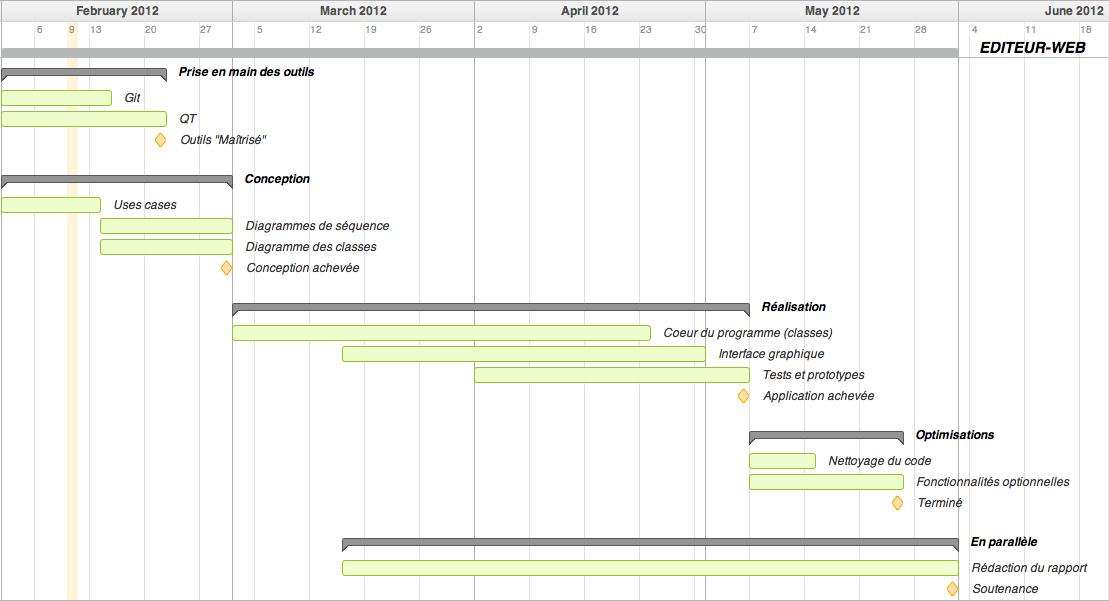
\includegraphics[width=17cm]{DiagrammeGantt.png}
						\caption{Diagramme de Gantt}
					\end{center}
				\end{figure}~\\
			\end{section}
		\end{chapter}
	\end{part}
\end{document}
